\documentclass[a4paper,11.5pt,onecolumn]{article}
\usepackage{graphicx,color}
\usepackage{amssymb} %math symbols
\usepackage{booktabs}%for nice tables
\usepackage{mathabx}%for \lesssim
\usepackage{pdfpages}%for cover page pdf import
\usepackage{draftwatermark}
\usepackage{hyperref}
\usepackage{natbib} %for citep and citet
\usepackage{float}

\floatstyle{boxed} 
\restylefloat{figure}
\hypersetup{colorlinks=true, linkcolor=blue, filecolor=blue, urlcolor=blue, citecolor=blue}
\pagestyle{empty}
\sloppy
\usepackage[left=2.2cm,top=2cm,right=1.8cm,bottom=2cm,nohead]{geometry}
\makeatletter
% \def\@seccntformat#1{}
\makeatother


\begin{document}
\bigskip
\bigskip
\title{Grassland update}
\author{Yann Chemin}
\maketitle
\bigskip
\bigskip
\section{Introduction}
Mars4Cast group is using a CAPRI-based project side product dating from 2000 as a grassland mask for all operations in MCYFS. There is a need for updating the mask with contemporary information while keeping resolution and homogeneity in the operational sytem. Of the most logical, pan-European homogeneous dataset of grassland, is the 2015 grassland product. The first section of this document is going to look into the details of this dataset, its characteristics and specifications to allow a better understanding of its use within an operational context in MCYFS. The second section of this document will look into some other sources of information, mostly from national sources, that have information about grass land or fodder harvesting.

\section{Copernicus GRASSLand products 2015}

The Copernicus grassland main product can be found in \citep{grassland2015} is dated from 2015, with a temporal frame period of $\pm 1$ year, thus effectively a range of 2014-2016. It has a spatial resolution of 20x20m (Figure~\ref{fig1}).

\begin{figure}[htbp]
\centering
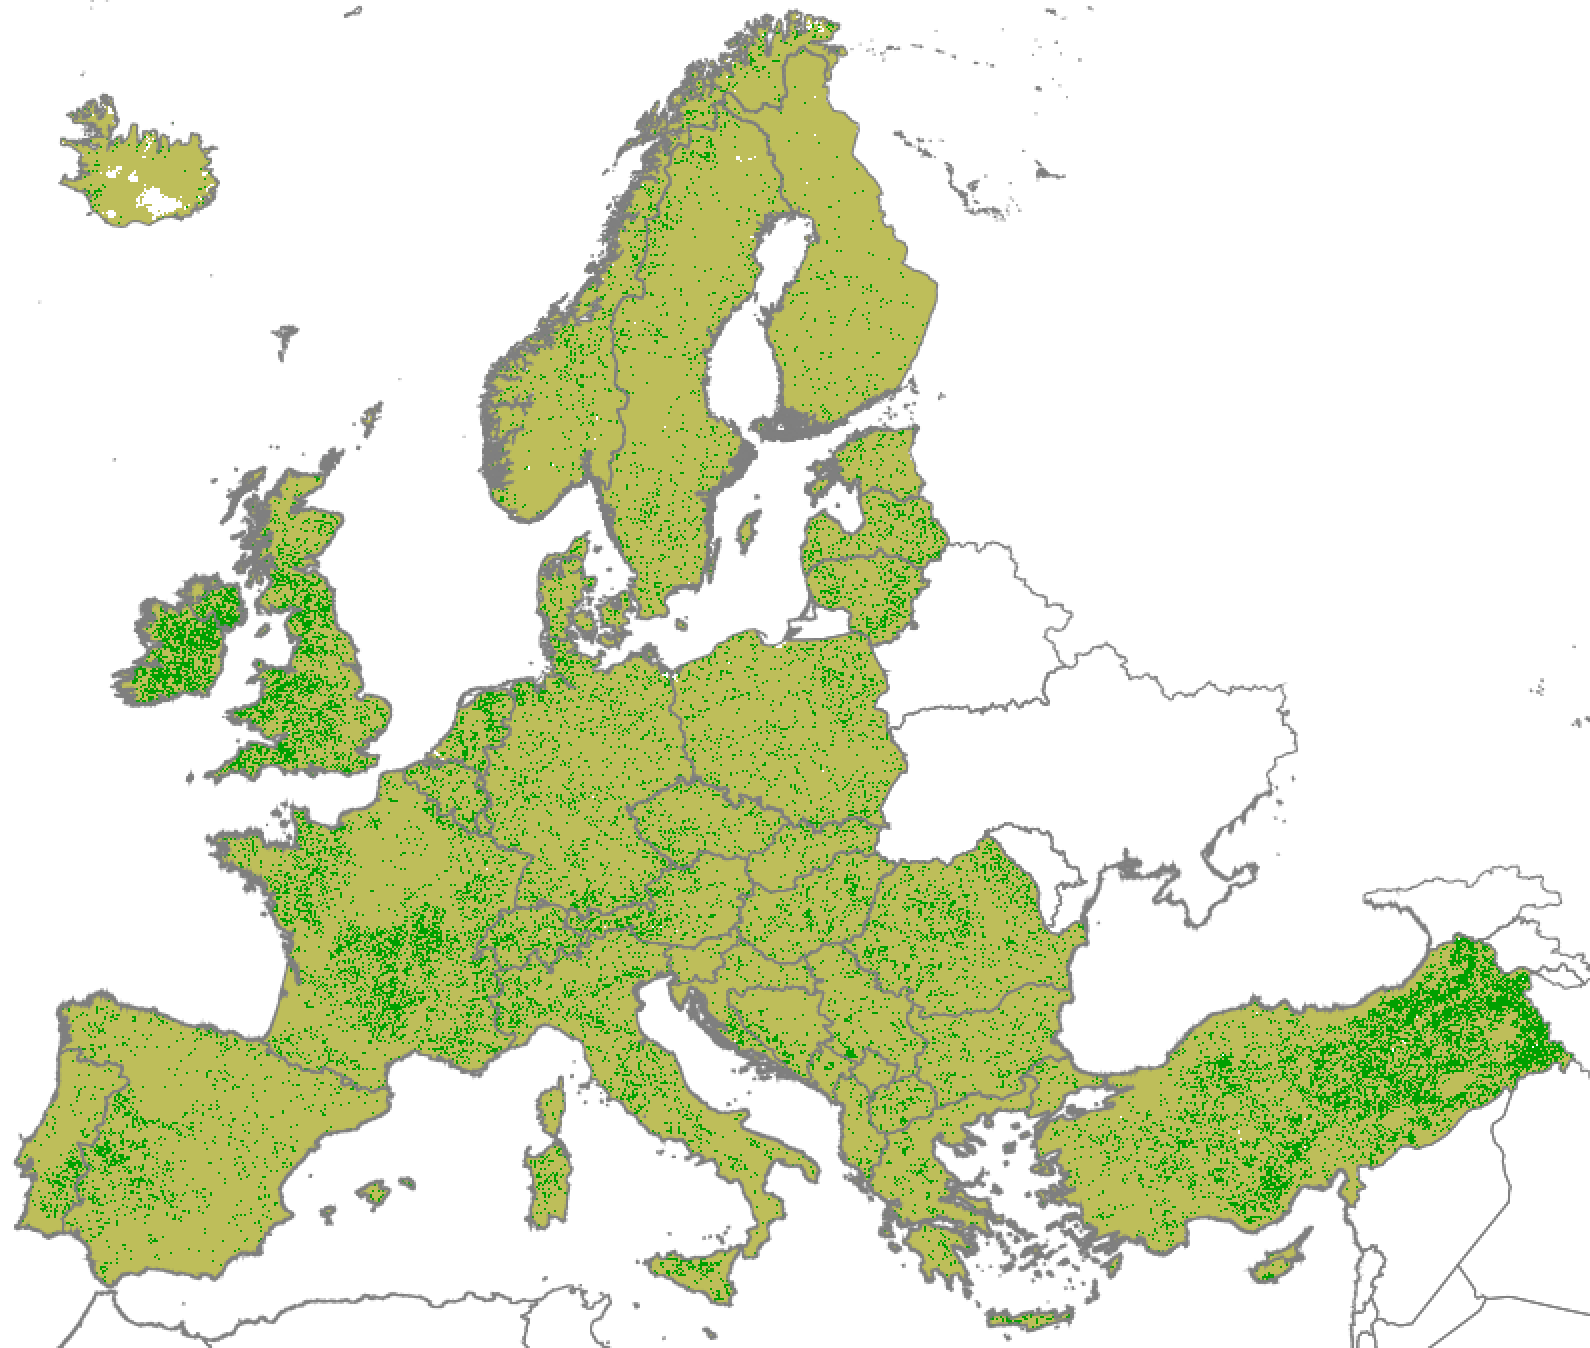
\includegraphics[width=0.85\textwidth]{images/grassland2015.png}
\caption{Copernicus Grassland product for 2015 (GRA\_2015\_020m\_eu\_03035\_V1\_4)}
\label{fig1}
\end{figure}

\noindent The effect of the spatial resolution can be found here on a zoom centered on Carnac/Quiberon, Western France (Figure~\ref{fig2}). Though the resolution is very good, the precision of grassland detection is not returning every permanent non-sown fields harvested yearly as general fodder, i.e. ``round balers''. As well as grassland fields falling under the littoral conservation Act \citep{france1986}.

\begin{figure}[htbp]
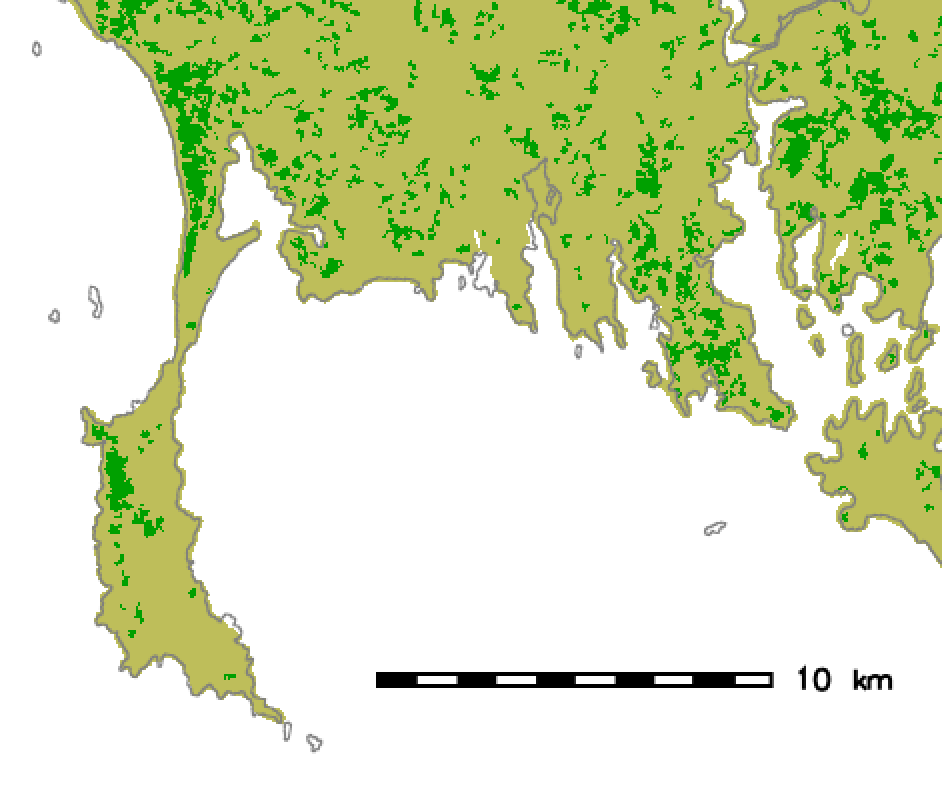
\includegraphics[width=0.85\textwidth]{images/grassland2015_zoom.png}
\caption{Copernicus Grassland product for 2015 (zoomed)}
\label{fig2}
\end{figure}

\noindent The base datasets used for the production are found in Figure~\ref{fig3}. As seen, the sources for auxiliary datasets are variable in type and time range. The specifications of the grassland 2015 dataset in terms of defining what is grassland and what is not grassland in the map produced are the following and found in original download URL \citep{grasslandreport2018}.\newline\linebreak

\noindent About half of the auxiliary data comes from the Copernicus high-resolution layers (HRL) source at 20x20m resolution for both 2012 \& 2015. It has tree cover density \citep{tcdreport2018}, forest type \citep{ftyreport2018}, imperviousness \citep{impreport2018}, water \& wet areas \citep{wwareport2018}.\newline\linebreak

\noindent The other half is variable, it hasEuropean/global datasets like the LUCAS ground truth dataset \citep{lucas2019}, the global forest cover dataset \citep{hansen2013high} and the Corine Land Cover \citep{corine2019}. Finally National datasets (LIPS, SIOSE) when available, as well as the German dataset of phenology PHASE.\newline\linebreak

\noindent In more detail, the grassland dataset encompasses the following features:
\begin{enumerate}
\item herbaceous vegetation $> 30\%$ ground cover, $> 30\%$ graminoid
species (Poaceae, Cyperaceae \& Juncaceae)
\item Possible scattered trees and shrubs, covering $< 10 \%$.
\item Possible non woody plants: lichens, mosses and ferns
\end{enumerate}

\begin{figure}[htbp]
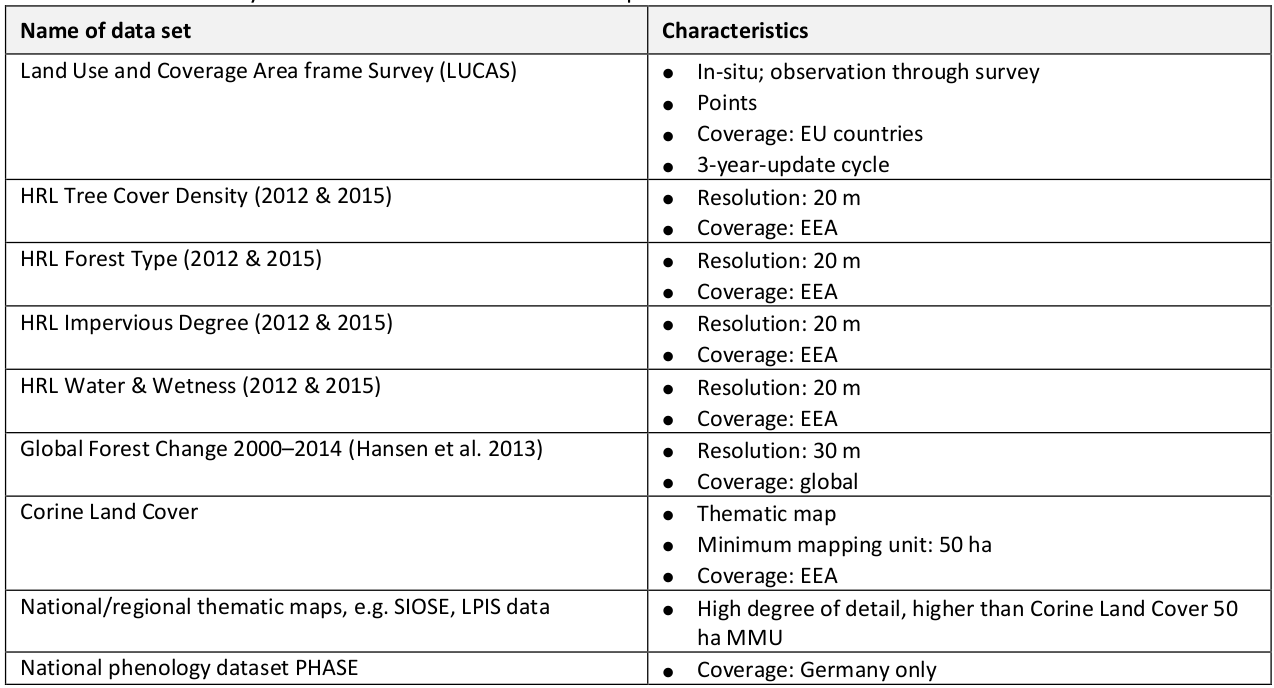
\includegraphics[width=\textwidth]{images/grassland2015auxdatasets.png}
\caption{Copernicus Grassland Auxiliary datasets used}
\label{fig3}
\end{figure}

\begin{figure}[htbp]
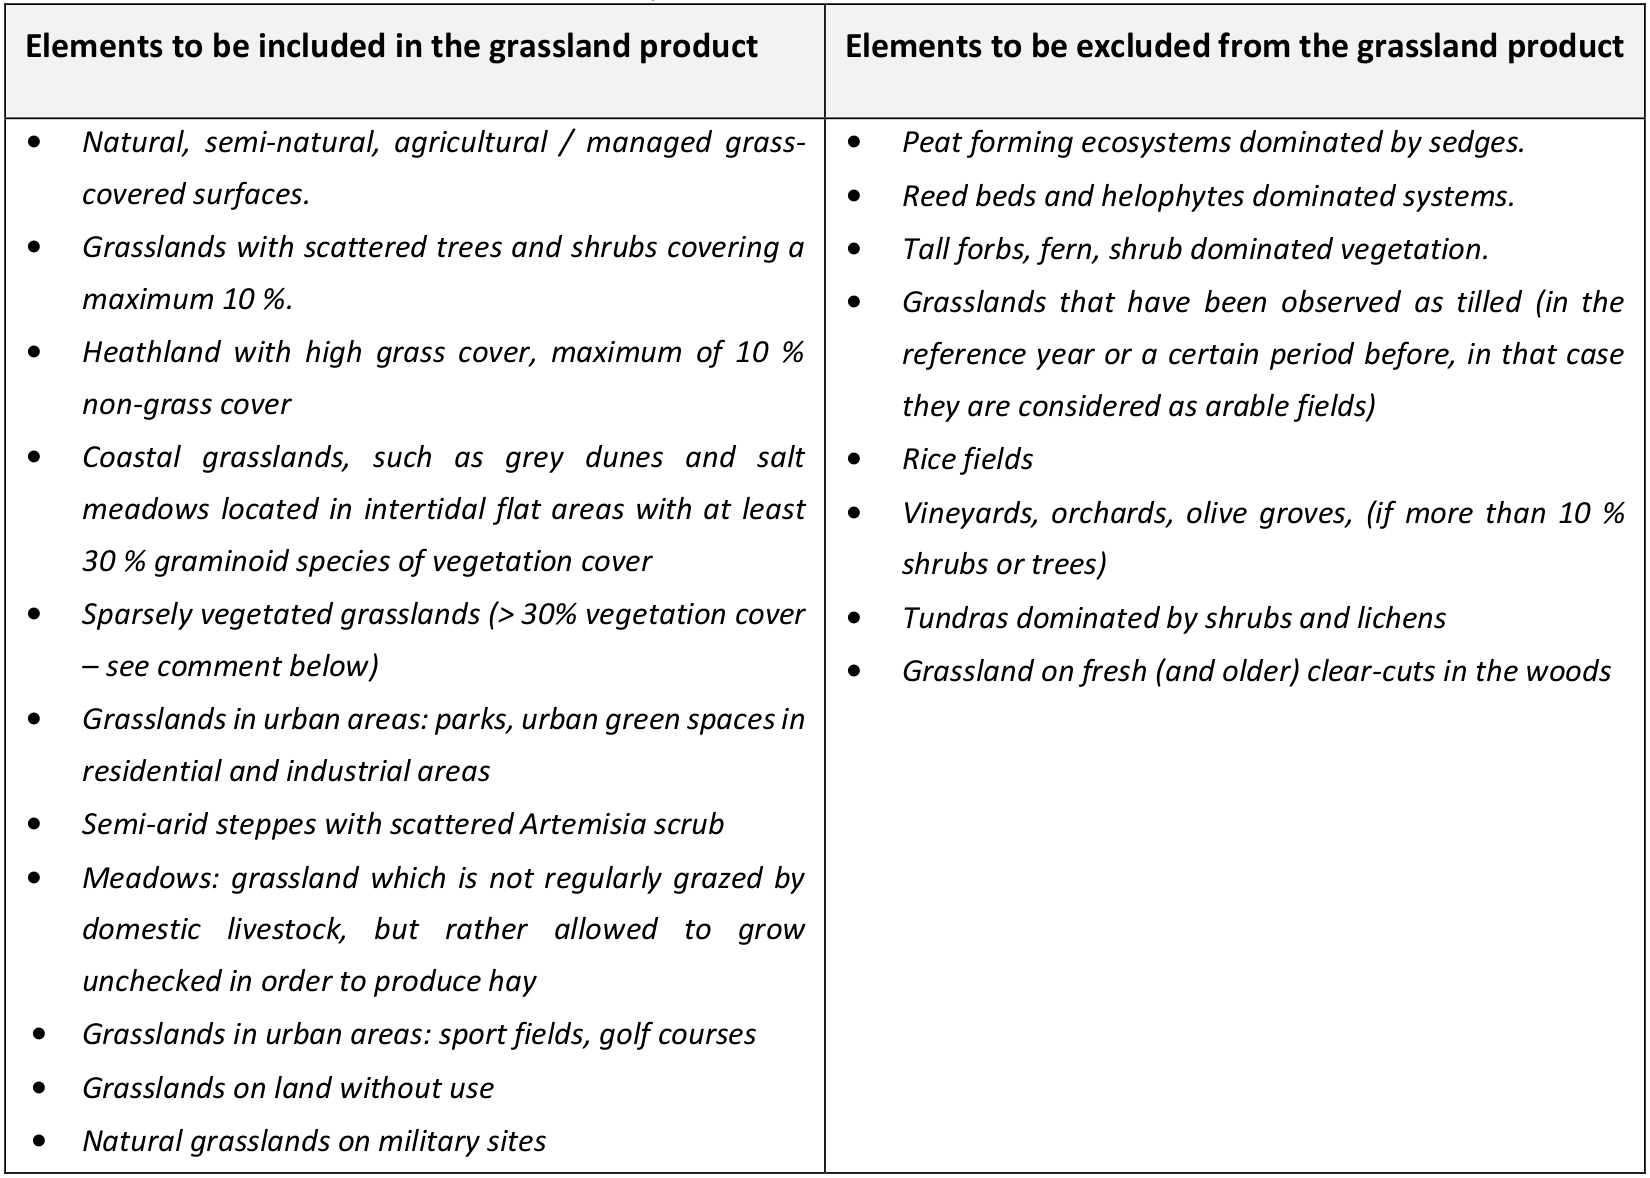
\includegraphics[width=\textwidth]{images/grasslanddefns.png}
\caption{Copernicus Grassland Definitions and exclusions}
\label{fig4}
\end{figure}

\newpage
\noindent The definitions included and excluded into the grassland product are found in Figure~\ref{fig4}. The main threshold used is the shrubs/trees $>10\%$, below that is considered grassland. This applies to vineyards, orchards, groves, tundras, woodland clear-cut, forbs, ferns. Halophytes and peat ecosystems are not incuded, as well as rice fields and tilled land.\newline\linebreak
\noindent Grassland is defined by several parameters. From the less vegetated side, drylands/tundras should have a minimum of $30\%$ of grass cover, in more temperate climates, grassland should cover $> 90\%$ of the area. An exclusion factor is the presence of tilling during a given amount of years prior to current. A dedicated product is defined to provide information on that. \textit{The Ploughing Indicator estimates the temporal extent since last ploughing activity. PLOUGH is
derived from historical bare soil time series (up to 6 years) of multi-temporal optical HR imagery} on a pixel-based, giving the latest bare soil indication, i.e. the number of years prior to the current year.\newline\linebreak
\noindent The Grass Vegetation Probability Index indicates to which degree
grassland could be separated from other vegetated land cover types $[1-100\%]$. Cloud is the main factor reducing multi-temporal classification accuracy.\newline\linebreak

\begin{figure}[htbp]
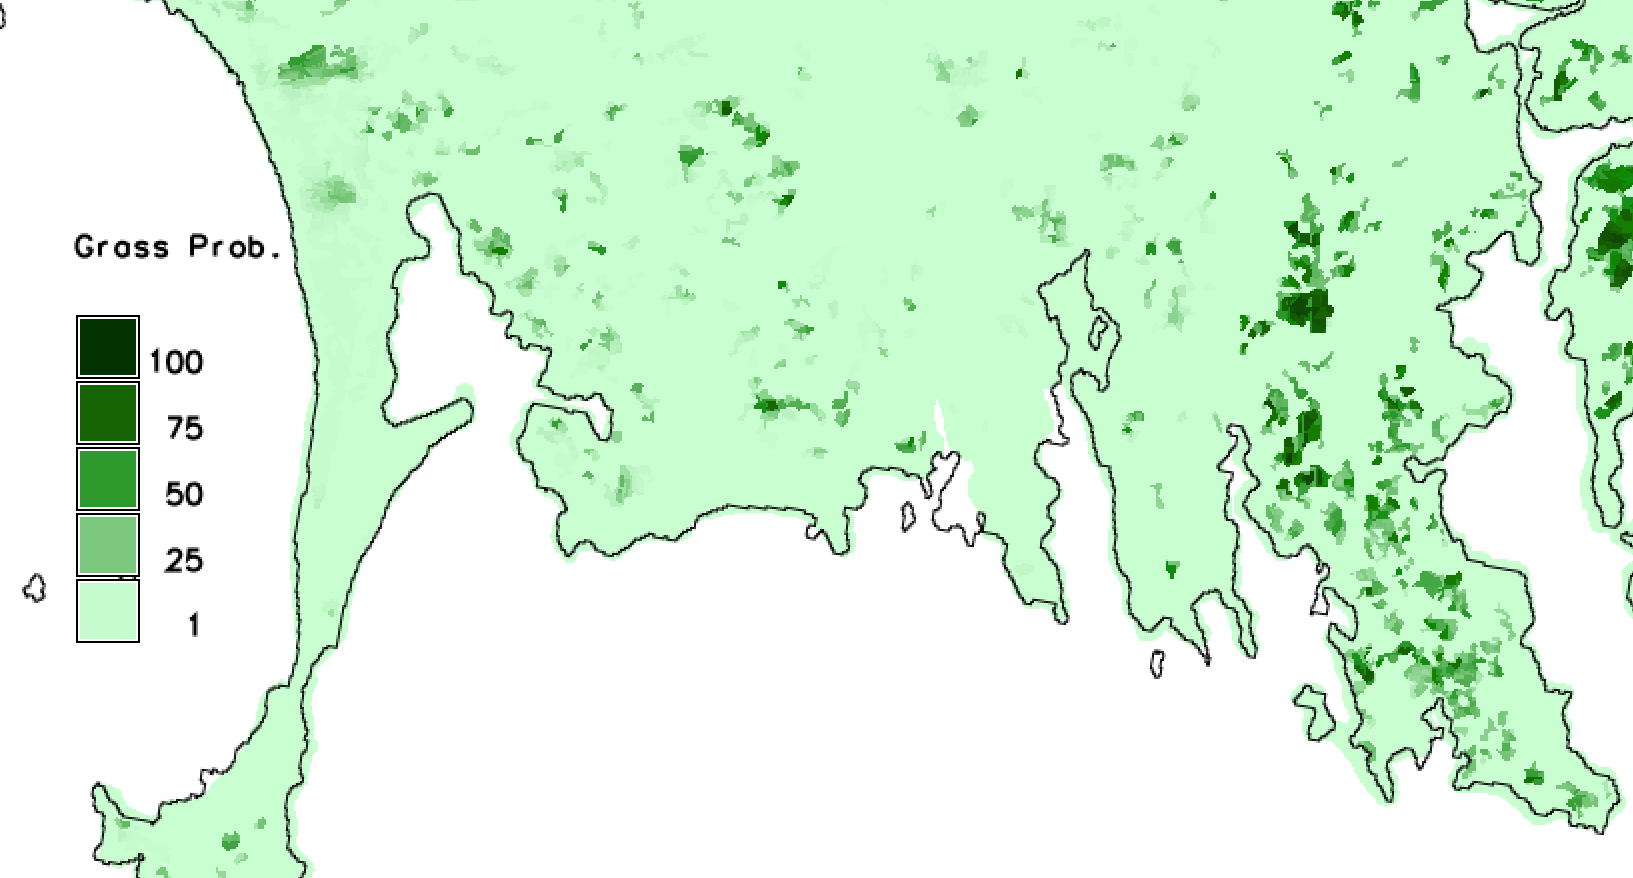
\includegraphics[width=\textwidth]{images/grasspvi_zoomed.png}
\caption{Copernicus Grassland Probability Index [0-100\%]}
\label{fig5}
\end{figure}

\section{Other products available}
\subsection{FR: Registre Parcellaire Graphique}
The \textit{Registre Parcellaire Graphique} is a repository of GIS data of reported agricultural fields for the purpose of the CAP subsidies. It is openly available online on a yearly basis with all agricultural crops within each parcel (\href{https://www.data.gouv.fr/en/datasets/registre-parcellaire-graphique-rpg-contours-des-parcelles-et-ilots-culturaux-et-leur-groupe-de-cultures-majoritaire/}{https://www.data.gouv.fr/en/datasets/registre-parcellaire-graphique-rpg-contours-des-parcelles-et-ilots-culturaux-et-leur-groupe-de-cultures-majoritaire/}). It does not cover all agricultural parcels in France, only the CAP subsidized ones. The official attributes definition gives 87 classes under fodder, not including maize as a fodder. Examples following show the presence of winter wheat\footnote{content is not related, but spatial and temporal dimensions indicated are, they were already made maps at the time of writing this document} integrated on 2010-2017, on all France (Figure~\ref{fig6}) and for the Southwestern part of Paris (Figure~\ref{fig7}).\newline\linebreak

\noindent Apparently, NL and DK have similar data available online. Maybe more countries have this for download, thus greatly improving the resolution of the information both in space and time (FR is yearly, with a 1 year delay after summer). 

\begin{figure}[htbp]
\begin{center}
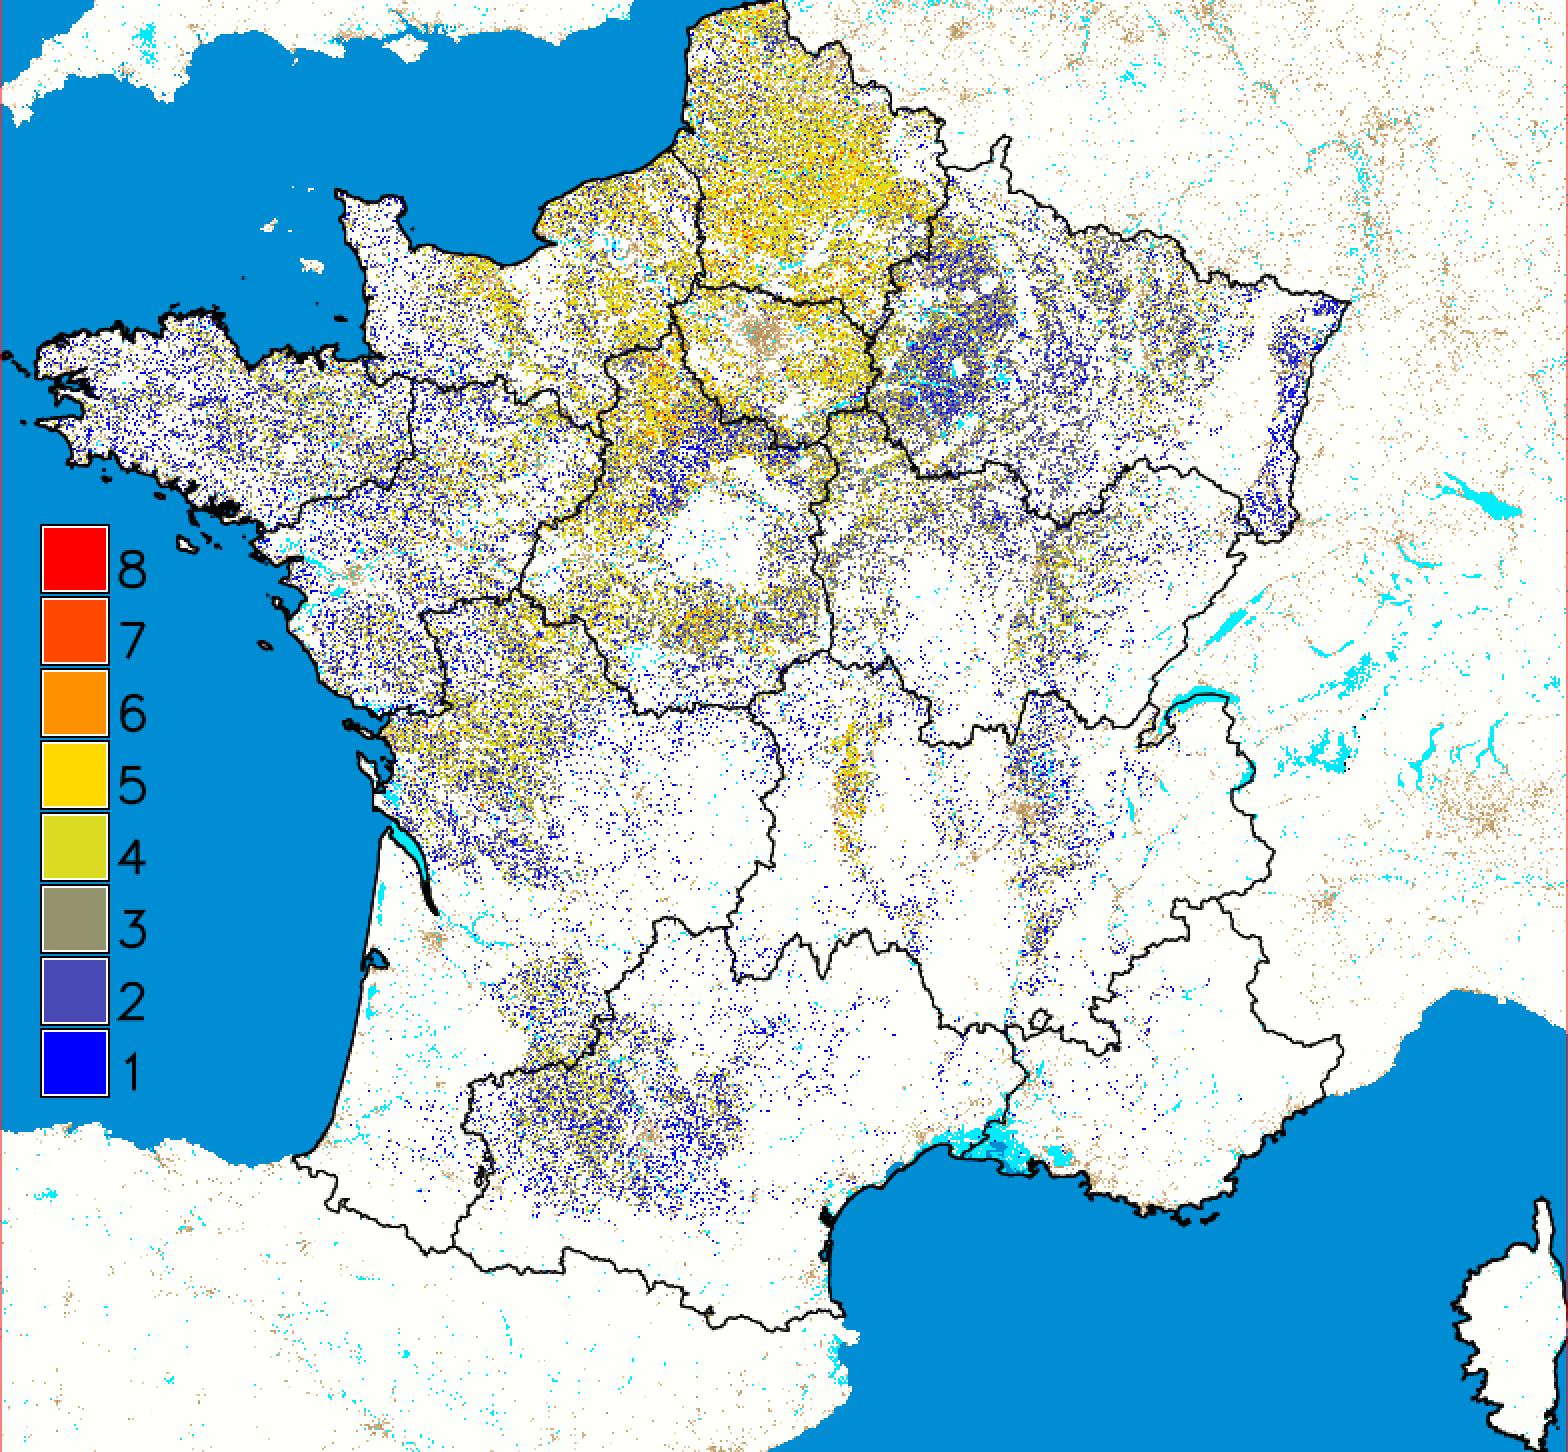
\includegraphics[width=0.60\textwidth]{images/RPG.png}
\caption{RPG Winter Wheat presence 2010-2017 (count) FR}
\end{center}
\label{fig6}
\end{figure}

\begin{figure}[htbp]
\begin{center}
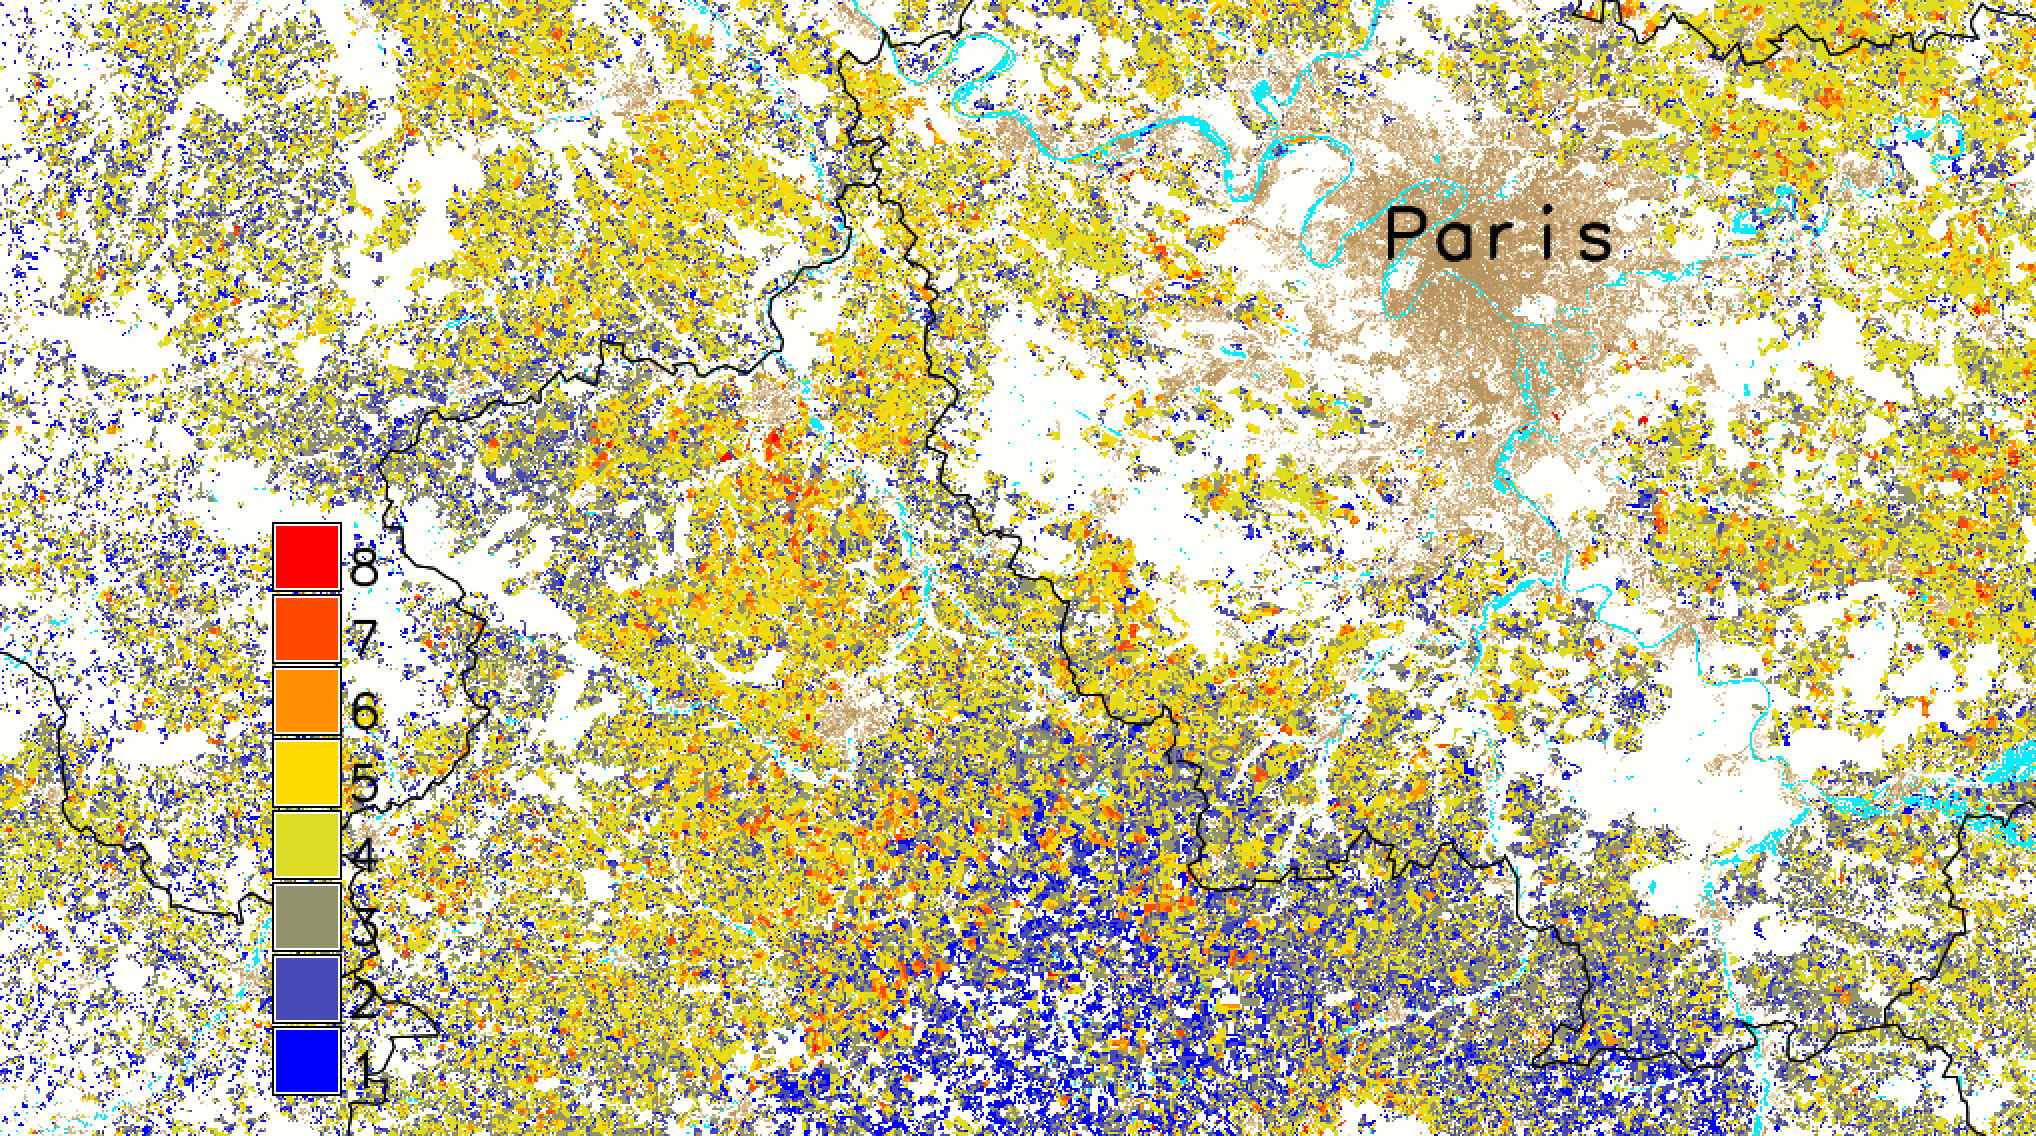
\includegraphics[width=0.82\textwidth]{images/RPG_zoomed.png}
\end{center}
\caption{RPG Winter Wheat presence 2010-2017 (count) SouthWest of Paris}
\label{fig7}
\end{figure}

\newpage
\section{Sentinel-1 IW SLC potential for grass-cut count}
\subsection{Meeting with the JEODPP}
A recent discussion with the JEODPP team (Dario R, Peter K, Tomas K on 5$^{th}$ of October 2019), highlighted the following facts:

\begin{enumerate}
\item Sentinel-1 is not downloaded as nobody uses it (but NL for Guido's)
\item Guido has given a script for preprocessing polarisation products to JEODPP
\item JEODPP is more than happy to (pre)process S1 images for MARS4CAST  
\end{enumerate}

Consequently, I have given a first set of countries to download the full archive of Sentinel-1: Portugal, Spain, France, Italy, Ukraine. As we have the yearly RPG (2010-2017) for France, we can use that to zero-in on the parcels of interest, and mask all non-parcels areas from processing/analysis. 

\subsection{Radar temporal coherence goal and potential use for MARS4CAST}
The temporal coherence tracks jumps in behaviour across time for a given area observed. It is a kind of complex (in both mathematical and real life meanings) diachronic difference mapping used in the common world of multi-spectral remote sensing.

When thinking about a grass cutting event, we can easily visualize a 50cm tall meadow with various species of several roughness, textures, colours, etc. That plant community on the paddock/meadows/fields ranges has a certain set of radar characteristics, and when the grass is cut, texture, roughness and the like change dramatically. The shorter the time between two observations, the brighter the difference (aka the coherence change, see Figure~\ref{fig8}).

\begin{figure}[htbp]
\begin{center}
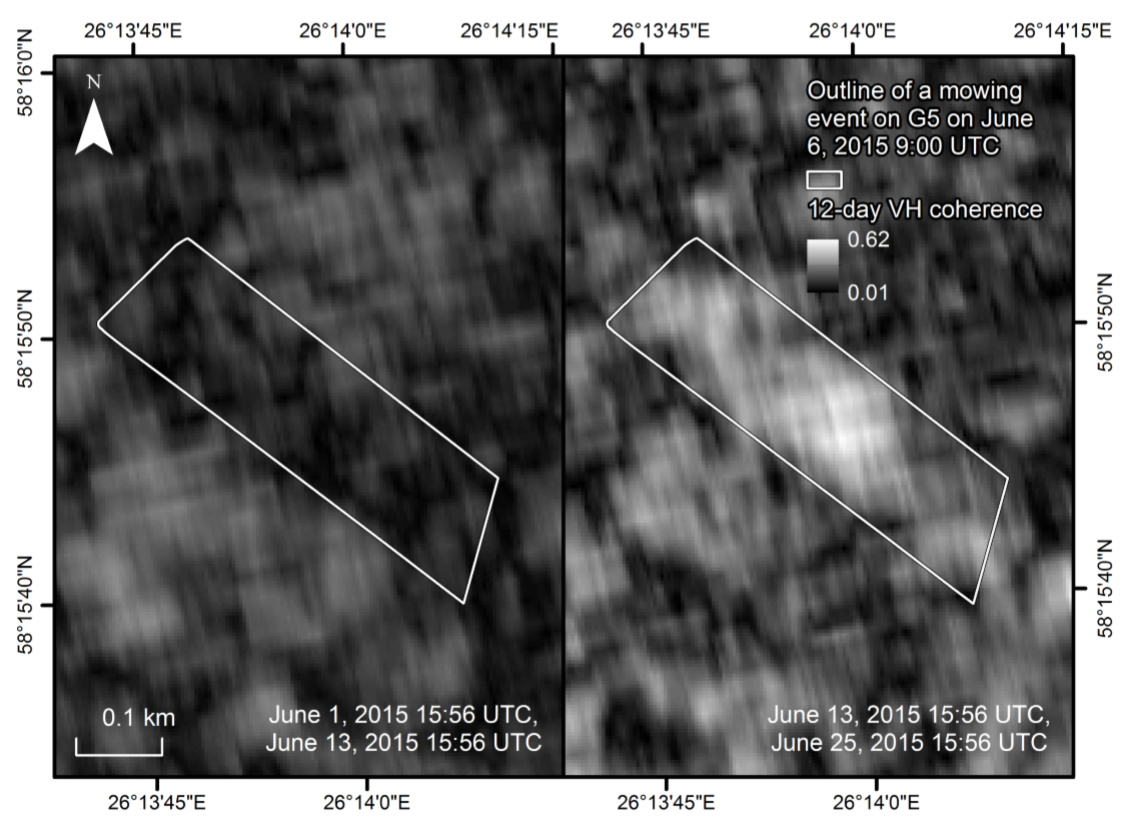
\includegraphics[width=0.9\textwidth]{images/S1GrassCutEventCoherence.png}
\end{center}
\caption{S1 12-day VH coherence before and after a mowing event 6 June 2015 \citep{tamm2016relating}}
\label{fig8}
\end{figure}

While those events can be assessed by Sentinel-1 on a 12 days diachronism for a single platform (i.e. Sentinel 1A) it can be reduced to 6 days if using both Sentinel 1A and 1B. Eventually, for a given temporal range (season/year), diachronic pairs can be assessed for coherence and a given number of cut can be estimated. Grass is cut 2-5 times a year depending on the function/use of the paddock.

As a corollary, not only grass cut maybe monitored, as main crops also have the harvesting cut event. Extraction of parcel areas across Europe (as available in France and The Netherlands actually, should permit to assess this primordial phenological event for fields across Europe. 

\subsection{Radar temporal coherence method and processing details}
The temporal coherence ($\gamma$) of two successive complex number bands of Sentinel-1 (IW-SLC) for a given moving window of area $n \times m$ is essentially the absolute of the complex conjugate product of the two temporally separated bands divided by the square root of the product of the single dates complex conjugate products on themselves. The coherence is \textit{thankfully} ranged from 0 to 1, with the value directly proportional to the coherence.

\begin{equation}
\gamma_{n \times m} = {|{\langle S_{t0}, S_{t1} \rangle|} \over \sqrt { \langle S_{t0}, S_{t0} \rangle  \langle S_{t1}, S_{t1} \rangle}} \quad 0 < \gamma < 1
\end{equation}

With $\langle x,y \rangle$ the complex conjugate product of x,y $\in \mathbb{C}$. Though the temporal coherence above seems a rather straightforward computation between two complex S1 images across time, there are several biases to the total coherence observed, in such a way that we have to redefine the temporal coherence within the influences of a group of coherences observed in what we can call the \textit{total coherence} $\gamma_{total}$ as follow for a given moving window:

\begin{equation}
\gamma_{total} = \gamma_{temporal} \times \gamma_{SNR} \times \gamma_{bias} \times  \gamma_{other}  
\end{equation}

While the $\gamma_{other}$ is considered an $\varepsilon$ element, the $\gamma_{bias}$ is directly proportional to the moving window area defined earlier as ($n \times m$). The largest contribution is thus the $\gamma_{SNR}$, the Signal-to-Noise-Ratio coherence across time defined below as:
 
\begin{equation}
\gamma_{SNR} = {1 \over {\sqrt{\left ( 1 + {1 \over {SNR_{S_{t0}}}}\right )\left ( 1 + {1 \over {SNR_{S_{t1}}}}\right )}}}  
\end{equation}

with $SNR_{S_{ti}}$, $i$ being the timestamp number, being defined as:

\begin{equation}
SNR_{S_{ti}} = { {\Gamma^o_{S_{ti}} - NESZ_{S_{ti}}} \over NESZ_{S_{ti}} }
\end{equation}

with $\Gamma^o_{sat}$ the backscattering coefficient of the moving window area $n \times m$ and $NESZ_{S_{ti}}$ the range dependent noise parameter, available in the Sentinel-1 metadata.To process coherence, few preprocessing steps are necessary to prepare the pairs of IW-SLC complex images. The full processing chain would be summarized by the following:

\begin{enumerate}
\item Application of precise orbit file (Figure~\ref{fig9})
\item Coregistration to sub-pixel accuracy with S1 TOPS Back Geocoding (Figure~\ref{fig10})
\item Compute coherence with removal of the flat earth phase term  (Figure~\ref{fig11})
\item Process polarisation in HV and VV for display support and other analyses
\end{enumerate}


\begin{figure}[htbp]
\begin{center}
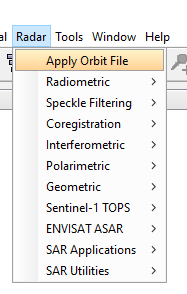
\includegraphics[width=0.3\textwidth]{images/SNAP_S1_Apply_Orbit_File}
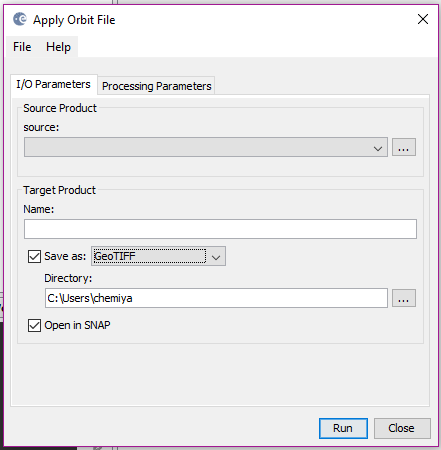
\includegraphics[width=0.6\textwidth]{images/SNAP_S1_Apply_Orbit_File_GUI}
\end{center}
\caption{SNAP S1 Orbit File Menu and GUI}
\label{fig9}
\end{figure}

\begin{figure}[htbp]
\begin{center}
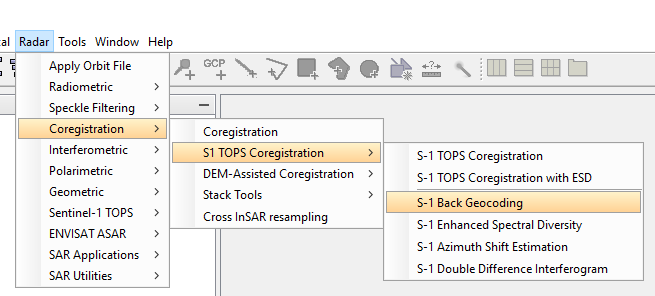
\includegraphics[width=0.65\textwidth]{images/SNAP_S1_Back_Geocoding}
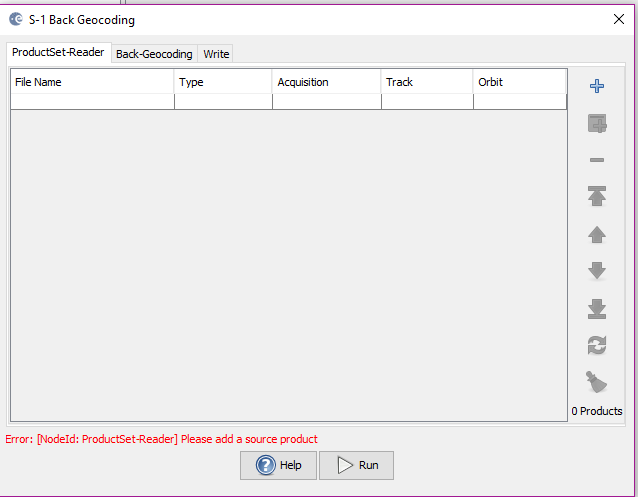
\includegraphics[width=0.6\textwidth]{images/SNAP_S1_Back_Geocoding_GUI}
\end{center}
\caption{SNAP S1 Back Geocoding Menu and GUI}
\label{fig10}
\end{figure}

\begin{figure}[htbp]
\begin{center}
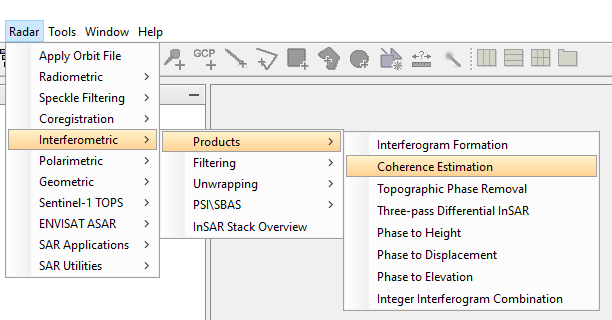
\includegraphics[width=0.65\textwidth]{images/SNAP_S1_Coherence}
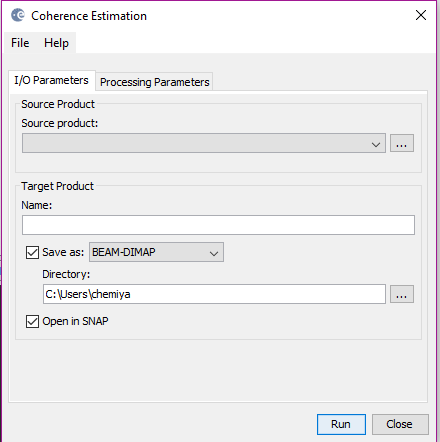
\includegraphics[width=0.48\textwidth]{images/SNAP_S1_Coherence_GUI}
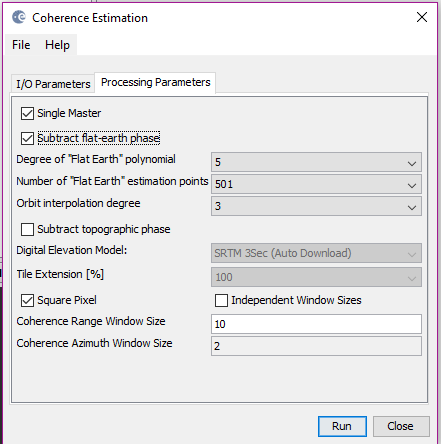
\includegraphics[width=0.48\textwidth]{images/SNAP_S1_Coherence_GUI_Params}
\end{center}
\caption{SNAP S1 Back Geocoding Menu and GUI}
\label{fig11}
\end{figure}

\newpage
%\bibliographystyle{authordate1}
%\bibliographystyle{plain}
\bibliographystyle{plainnat}
%\bibliographystyle{abbrv}
%\bibliographystyle{acm}
%\bibliographystyle{nar}
%\bibliographystyle{alpha}
%\bibliographystyle{amsplain}
%\bibliographystyle{amsalpha}
\bibliography{LaTex_20190704_JRC_Grassland}


\end{document}
